% !TEX root = thesis.tex

\chapter{A reoccurring pattern}

First I introduce the pattern that forms the focus of the first part of the dissertation. I show that headless relatives in Gothic adhere to the case strength scale: \ac{nom} < \ac{acc} < \ac{dat}.

Then I show two phenomena that follow the same ordering of \ac{nom}, \ac{acc} and \ac{dat}. The two phenomena are accessibility hierarchies. The first one is about agreement, the second one about relativization.

In the last section of this chapter I discuss how \ac{nom}, \ac{acc} and \ac{dat} pattern in morphology.


\section{Case competition in Gothic headless relatives}

In this section I show the behavior of Gothic headless relatives in detail. I systematically go through all case combinations, except for the genitive, to which I return in Section \ref{sec:genitive}. This leaves the nominative, accusative and dative. First, I discuss the matching headless relatives, in which the internal and external case match.

Consider the example in \ref{ex:gothicaccaccrep}, repeated from the introduction. In this example, the internal case and the external case are accusative.
The relative clause, including the relative pronoun, is marked in gray.
The internal case is accusative. The predicate \tit{arma} `pity' takes accusative objects.
The external case is accusative as well. Here the predicate \tit{gaarma} `pity' takes accusative objects.
The relative pronoun \tit{þan(a)} `who.\ac{acc}' appears in the accusative.

\exg. gaarma \tcol{DG}{þan} \tcol{DG}{-ei} \tcol{DG}{arma}\\
 pity\scsub{[acc]} who.\ac{acc} -\ac{comp} pity\scsub{[acc]}\\
 `I will pity (him) whom I pity' \flushfill{Gothic, \ac{rom} 9:15, after \pgcitealt{harbert1978}{339}}\label{ex:gothicaccaccrep}

 Consider the example in \ref{ex:gothicnomnom}, in which the internal case and the external case are nominative.
 The relative clause, including the relative pronoun, is marked in gray.
 The internal case is nominative. The predicate \tit{matjai} `eats' takes nominative subjects.
 The external case is nominative as well. Here the predicate \tit{gadauþnai} `die' takes nominative subjects.
 The relative pronoun \tit{sa} `who.\ac{nom}' appears in the nominative.

\exg. ei \tcol{DG}{sa} \tcol{DG}{-ei} \tcol{DG}{þis} \tcol{DG}{matjai}, ni gadauþnai\\
 that who.\ac{nom} -\ac{comp} {of this} eats\scsub{[nom]} not die\scsub{[nom]}\\
 `that (he) who eats of this may not die' \flushfill{Gothic, \ac{john} 6:50, after \pgcitealt{harbert1978}{337}}\label{ex:gothicnomnom}

 Consider the examples in \ref{ex:gothicdatdat}, in which the internal case and the external case are dative.
 The relative clauses, including the relative pronoun, is marked in gray.
 The internal case is dative. The predicates \tit{gabaur} `tribute', \tit{mota} `custom', \tit{agis} `fear' and \tit{sweriþa} `honour' takes dative objects.
 The external case is dative as well. The same predicates as in the relative clause take dative objects.
 The relative pronouns \tit{þamm(a)} `who.\ac{dat}' appear in the dative.

\ex.\label{ex:gothicdatdat}
\ag. \tcol{DG}{þamm} \tcol{DG}{-ei} \tcol{DG}{gabaur} gabaur\\
 who.\ac{dat} -\ac{comp} tribute\scsub{[dat]} tribute\scsub{[dat]}\\
 `tribute to (him) whom tribute is due'
\bg. \tcol{DG}{þamm} \tcol{DG}{-ei} \tcol{DG}{mota} mota\\
 \tcol{DG}{who.\ac{dat}} \tcol{DG}{-\ac{comp}} \tcol{DG}{custom\scsub{[dat]}} custom\scsub{[dat]}\\
 `custom to (him) whom custom is due'
\bg. \tcol{DG}{þamm} \tcol{DG}{-ei} \tcol{DG}{agis} agis\\
 \tcol{DG}{who.\ac{dat}} \tcol{DG}{-\ac{comp}} \tcol{DG}{fear\scsub{[dat]}} fear\scsub{[dat]}\\
 `fear (him) whom fear is due'
\bg. \tcol{DG}{þamm} \tcol{DG}{-ei} \tcol{DG}{sweriþa} sweriþa\\
 \tcol{DG}{who.\ac{dat}} \tcol{DG}{-\ac{comp}} \tcol{DG}{honour\scsub{[dat]}} honour\scsub{[dat]}\\
 `honour (him) whom honour is due' \flushfill{Gothic, \ac{rom} 13:7, after \pgcitealt{harbert1978}{339}}

A summary of data so far is given in Table \ref{tbl:summarygothicmatch}. The left column shows the internal case between square brackets. The upper row shows the external case between square brackets. The other cells indicate the case of the relative pronoun.
So far only the diagonal line is filled. These are the matching examples, the examples in which the internal case matches the external case. The relative pronoun appears in the internal and external case, and it is marked in dark gray. The nominative is given in \ref{ex:gothicnomnom}, the accusative in \ref{ex:gothicaccaccrep}, and the dative in \ref{ex:gothicdatdat}.

\begin{table}[H]
  \center
  \caption {Summary of Gothic matching headless relative data}
    \begin{tabular}{c|c|c|c}
      \toprule
        \diagbox[linecolor=white]{\ac{int}}{\ac{ext}}
            & [\ac{nom}]
            & [\ac{acc}]
            & [\ac{dat}]
            \\ \cmidrule{1-4}
        [\ac{nom}]
            & \colorbox{LG}{\ac{nom}}
            & \diagbox[linecolor=white]{\phantom{nom}}{\phantom{nom}}
            & \diagbox[linecolor=white]{\phantom{nom}}{\phantom{nom}}
            \\ \cmidrule{1-4}
        [\ac{acc}]
            & \diagbox[linecolor=white]{\phantom{nom}}{\phantom{nom}}
            & \colorbox{LG}{\ac{acc}}
            & \diagbox[linecolor=white]{\phantom{nom}}{\phantom{nom}}
            \\ \cmidrule{1-4}
        [\ac{dat}]
            & \diagbox[linecolor=white]{\phantom{nom}}{\phantom{nom}}
            & \diagbox[linecolor=white]{\phantom{nom}}{\phantom{nom}}
            & \colorbox{LG}{\ac{dat}}
            \\
      \bottomrule
    \end{tabular}
    \label{tbl:summarygothicmatch}
\end{table}

In what follows, I discuss the non-matching headless relatives, in which the internal and external case differ.

Consider the example in \ref{ex:gothicnomacc}, in which the internal case is nominative and the external case is accusative.
The relative clause, excluding the relative pronoun, is marked in gray.
The internal case is nominative. The predicate \tit{ist us Laudeikaion} `is from Laodicea' takes nominative subjects.
The external case is accusative. The predicate \tit{ussiggwaid} `read' takes accusative objects.
The relative pronoun \tit{þo} `what.\ac{acc}' appears in the external case: the accusative.
Examples, in which the relative pronoun appears in nominative case, the internal case is nominative and the external case is accusative, are unattested.

\exg. jah þo \tcol{DG}{-ei} \tcol{DG}{ist} \tcol{DG}{us} \tcol{DG}{Laudeikaion} jus ussiggwaid\\
 and what.\ac{acc} -\ac{comp} is\scsub{[nom]} from Laodicea you read\scsub{[acc]}\\
 `and read that which is from Laodicea' \flushfill{Gothic, \ac{col} 4:16, after \pgcitealt{harbert1978}{357}}\label{ex:gothicnomacc}

Consider the example in \ref{ex:gothicnomdat}, in which the internal case is nominative and the external case is dative.
The relative clause, excluding the relative pronoun, is marked in gray.
The internal case is nominative. The predicate \tit{sind fraþjaiþ} `are above' takes a nominative subject.
The external case is dative. The predicate \tit{fraþjaiþ} `think on' takes dative indirect objects.
The relative pronoun \tit{þaim} `what.\ac{dat}' appears in the external case: the dative.
Examples, in which the relative pronoun appears in nominative case, the internal case is nominative and the external case is dative, are unattested.

\exg. þaim \tcol{DG}{-ei} \tcol{DG}{iupa} \tcol{DG}{sind} fraþjaiþ \\
 what.\ac{dat} -\ac{comp} above are\scsub{[nom]} {think on}\scsub{[dat]}\\
 `set your mind on those which are above' \flushfill{Gothic, \ac{col} 3:2, after \pgcitealt{harbert1978}{339}}\label{ex:gothicnomdat}

Consider the example in \ref{ex:gothicaccnom}, in which the internal case is accusative and the external case is nominative.
The relative clause, including the relative pronoun, is marked in gray.
The internal case is accusative. The predicate \tit{frijos} `love' takes accusative objects.
The external case is nominative. The predicate \tit{siuks ist} `is sick' takes nominative subjects.
The relative pronoun \tit{þan} `who.\ac{acc}' appears in the internal case: the accusative.
Examples, in which the relative pronoun appears in nominative case, the internal case is accusative and the external case is nominative, are unattested.

\exg. \tcol{DG}{þan} \tcol{DG}{-ei} \tcol{DG}{frijos} siuks ist\\
 who.\ac{acc} -\ac{comp} love\scsub{[acc]} sick is\scsub{[nom]}\\
 `the one whom you love is sick' \flushfill{Gothic, \ac{john} 11:3, after \pgcitealt{harbert1978}{342}}\label{ex:gothicaccnom}

Consider the example in \ref{ex:gothicaccdatrep}, repeated from the introduction. In this example, the internal case is accusative and the external case is dative.
The relative clause, excluding the relative pronoun, is marked in gray.
The internal case is accusative. The predicate \tit{qiþiþ} `say' takes accusative objects.
The external case is dative. The predicate \tit{taujau} `do' takes dative indirect objects.
The relative pronoun \tit{þamm} `who.\ac{dat}' appears in the external case: the dative.
Examples, in which the relative pronoun appears in accusative case, the internal case is accusative and the external case is dative, are unattested.

\exg. hva nu wileiþ ei taujau þamm \tcol{DG}{-ei} \tcol{DG}{qiþiþ} \tcol{DG}{þiudan} \tcol{DG}{Iudaie}?\\
 what now want that do\scsub{[dat]} who.\ac{dat} -\ac{comp} say\scsub{[acc]} king {of Jews}\\
 `what now do you wish that I do to (him) whom you call King of the Jews?' \flushfill{Gothic, \ac{mark} 15:12, after \pgcitealt{harbert1978}{339}}\label{ex:gothicdataccrep}

Consider the example in \ref{ex:gothicdatnom}, in which the internal case is dative and the external case is nominative.
The relative clause, including the relative pronoun, is marked in gray.
The internal case is dative. The predicate \tit{fraletada} `is forgiven' takes dative objects.
The external case is nominative. The predicate \tit{frijod} `loves' takes nominative subjects.
The relative pronoun \tit{þamm(a)} `who.\ac{dat}' appears in the internal case: the dative.
Examples, in which the relative pronoun appears in nominative case, the internal case is dative and the external case is nominative, are unattested.

\exg. iþ þamm -ei leitil fraletada leitil frijod\\
 but \tcol{DG}{who.\ac{dat}} \tcol{DG}{-\ac{comp}} \tcol{DG}{little} \tcol{DG}{{is forgiven}\scsub{[dat]}} little loves\scsub{[nom]}\\
 `but the one whom little is forgiven loves little' \flushfill{Gothic, \ac{luke} 7:47, after \pgcitealt{harbert1978}{342}}\label{ex:gothicdatnom}

Consider the example in \ref{ex:gothicdataccrep}, repeated from the introduction. In this example, the internal case is dative and the external case is accusative.
The relative clause, including the relative pronoun, is marked in gray.
The internal case is dative. The preposition \tit{ana} `on' takes dative complements.
The external case is accusative. The predicate \tit{ushafjands} `picking up' takes accusative objects.
The relative pronoun \tit{þamm(a)} `who.\ac{dat}' appears in the internal case: the dative.
Examples, in which the relative pronoun appears in accusative case, the internal case is dative and the external case is accusative, are unattested.

\exg. ushafjands ana þamm -ei lag\\
 {picking up}\scsub{[acc]} \tcol{DG}{on\scsub{[dat]}} \tcol{DG}{what.\ac{dat}} \tcol{DG}{-\ac{comp}} \tcol{DG}{lay}\\
 `picking up (that) on which he lay' \flushfill{Gothic, \ac{luke} 5:25, after \pgcitealt{harbert1978}{343}}\label{ex:gothicaccdatrep}

A summary of the Gothic data as a whole is given in Table \ref{tbl:summarygothic}. The left column shows the internal case, the upper row shows the external case. The diagonal is filled with matching examples, marked dark gray.
The remaining six cells show instances where the internal and external case differ. Within the cells, two cases are given. The case in the lower left corner stands for the relative pronoun in the internal case. The case in the upper right corner stands for the relative pronoun in the external case. The grammatical examples are marked in light gray. The unattested examples are marked with an asterix and are unmarked.\footnote{
Throughout this dissertation * stands for 'not found in natural language'. For extinct languages this means that there are no attested examples. For modern languages it means that the examples are ungrammatical.
}

\begin{table}[H]
  \center
  \caption {Summary of Gothic headless relative data}
    % !TEX root = ../thesis.tex

\begin{tabular}{c|c|c|c}
  \toprule
    \diagbox[linecolor=white]{\ac{int}}{\ac{ext}}
        & [\ac{nom}]
        & [\ac{acc}]
        & [\ac{dat}]
        \\ \cmidrule{1-4}
    [\ac{nom}]
        & 
        & \diagbox[linecolor=white]{*\ac{nom}}{\colorbox{LG}{\ac{acc}}}
        & \diagbox[linecolor=white]{*\ac{nom}}{\colorbox{LG}{\ac{dat}}}
        \\ \cmidrule{1-4}
    [\ac{acc}]
        & \diagbox[linecolor=white]{\colorbox{LG}{\ac{acc}}}{*\ac{nom}}
        &
        & \diagbox[linecolor=white]{*\ac{acc}}{\colorbox{LG}{\ac{dat}}}
        \\ \cmidrule{1-4}
    [\ac{dat}]
        & \diagbox[linecolor=white]{\colorbox{LG}{\ac{dat}}}{*\ac{nom}}
        & \diagbox[linecolor=white]{\colorbox{LG}{\ac{dat}}}{*\ac{acc}}
        &
        \\
  \bottomrule
\end{tabular}

    \label{tbl:summarygothic}
\end{table}

The three instances in the lower left corner correspond to the examples \ref{ex:gothicaccnom}, \ref{ex:gothicdatnom} and \ref{ex:gothicdataccrep}. In the attested examples, the relative pronoun appears in the internal case.
The three instances in the upper right corner correspond to the examples in \ref{ex:gothicnomacc}, \ref{ex:gothicnomdat} and \ref{ex:gothicaccdatrep}. In the attested examples, the relative pronoun appears in the external case.

This can be reformulated as follows. In a competition, dative wins over accusative and nominative. This can be seen in the lowest row and the most right column. Additionally, accusative wins over nominative. In sum, the situation can be summarized as in \ref{ex:competition1by1}.

\ex.\label{ex:competition1by1}
\a. \tsc{acc} wins over \tsc{nom}
\b. \tsc{dat} wins over \tsc{nom}
\b. \tsc{dat} wins over \tsc{acc}

Formulated in a scale of `case strength' \citealt{harbert1978,pittner1995,vogel2001,grosu2003,caha2019}:

\ex. \tsc{nom} < \tsc{acc} < \tsc{dat}\label{ex:casestrength}

In the next few sections I show that this scale of case strength does not only appear in headless relatives. The next section shows two other morphosyntactic phenomena that follow the same scale. Section \ref{sec:casemorphology} shows how the case scale is reflected in morphophonology.


\section{Parallels in accessibility hierarchies}

In this section I discuss two additional phenomena in morphosyntax that reflect the \tsc{nom} < \tsc{acc} < \tsc{dat} ordering.

\subsection{Agreement}

% The hierarchy is to be read as follows: if a language allows the verb to agree with an argument marked by a case X, it also allows the verb to agree with all arguments to the left of X.
%
% Moravcsik (1974) presented a set of implicational universals regarding (NP-predicate) agreement. The universals are formulated in terms of grammatical functions (subject, object, etc.), and include implicational hierarchy schematized in (12). The hierarchy ranges over languages, not sentences, and conflates a set of statements such as the following (see Moravcsik 1978 for revisions):
% • If in a language the verb agrees with anything, it agrees with some or all subjects
% • If the verb agrees with anything other than subjects, it agrees with some or all direct objects

\begin{figure}[H]
  \centering
  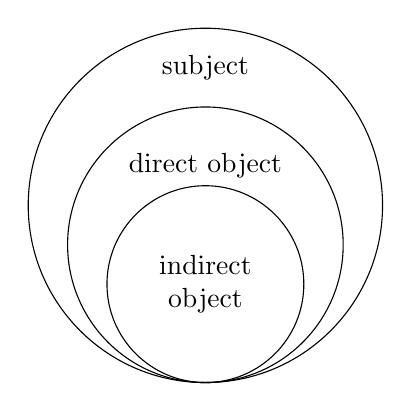
\begin{tikzpicture}
    \draw (0,1) circle (2.25);
    \draw (0,0.5) circle (1.75);
    \draw (0,0) circle (1.25);

    \node[] at (0,2.75) {subject};
    \node[] at (0,1.5) {direct object};
    \node[align=center] at (0,0) {indirect\\ object};
  \end{tikzpicture}
  \caption{\posscitealt{moravcsik1978} schema}
  \label{fig:subdoio}
\end{figure}


\citealt{moravcsik1978} with subject, object and indirect object.

Mandarin Chinese is an example of a language that does not show any agreement on the predicate. An example is given in \ref{ex:chineseagr}. The predicate \tit{gěi} `give' does not agree with the subject \tit{nǐ} `you', with the direct object \tit{shū} `book' or with the indirect object \tit{wǒ} `me'.

\exg. Nǐ bǎ shū gěi wǒ -le.\\
 you ba book give me -\ac{asp}\\
 `You gave me the book.' \flushfill{Mandarin Chinese, Zheng Shen p.c.}\label{ex:chineseagr}

German is an example of a language that shows agreement with the subject of the clause. An example is given in \ref{ex:germanagr}. The predicate \tit{gibst} `give' contains the morpheme \tit{-st}. This morpheme is the agreement morpheme for second person singular subjects. The predicate \tit{gibst} `give' agrees in person and number with the subject \tit{du} `you'. There is no agreement with the direct object \tit{das Buch} `the book' or the indirect object \tit{mir} `me'.

\exg. Du gib -st mir das Buch.\\
 you give -\tbf{2\ac{sg}} me the book\\
 `You give me the book.' \flushfill{German}\label{ex:germanagr}

Hungarian is an example of a language that shows agreement with the subject and the direct object of a clause. An example is given in \ref{ex:hungarianagr}. The predicate \tit{adom} `give' contains the morpheme \tit{-om}. This is a portmonteau morpheme for a first person singular subject and a third person object agreement. The predicate \tit{adom} `give' agrees with the subject \tit{én} `I' and the direct object \tit{a könyvet} `the book'. There is no agreement with the indirect object \tit{neked} `you'.

\exg. (Én) neked ad -om a könyv -et\\
 I you.\tsc{dat}.\tsc{sg} give -\tbf{\tsc{1sg}.\tsc{sbj}>3.\tsc{obj}} the book -\tsc{acc}\\
 `I give you the book.' \flushfill{Hungarian, András Bárány p.c.}\label{ex:hungarianagr}

Basque is an example of language that shows agreement with the subject, the direct object and the indirect object. An example is given in \ref{ex:basqueagr}. The auxiliary consists of the morphemes \tit{d-}, \tit{-austa} and \tit{-zu}. The morpheme \tit{d-} agrees with the direct object \tit{liburua} `the book'. The morpheme \tit{-austa} agrees with the indirect object \tit{niri} `me'. The morpheme \tit{-zu} agrees with the subject \tit{zuk} `you'.

\exg. Zu -k ni -ri liburu -a emon d -austa -zu.\\
 you -\ac{erg} me -\ac{dat} book -\ac{def}.\ac{acc} given \tbf{\ac{acc}.3\ac{sg}} \tbf{-\ac{dat}.1\ac{sg}} \tbf{-\ac{erg}.2\ac{sg}}\\
 `You gave me the book.' \flushfill{Basque, \pgcitealt{arregi2004}{45}}\label{ex:basqueagr}

\posscitealt{gilligan1987} typological study confims the picture.

 \begin{table}[H]
   \center
   \caption {Agreement accessibility}
     \begin{tabular}[t]{ccccc}
       \toprule
             \multicolumn{3}{c}{agreement with}
             &
           & \\
       \cmidrule{1-3}
             & direct
             & indirect
             & number
           & \\
             subject
             & object
             & object
             & of languages
           & example \\
       \cmidrule{1-3} \cmidrule{4-4} \cmidrule{5-5}
             *
             & *
             & *
             & 23
           & Mandarin Chinese \\
             ✔
             & *
             & *
             & 31
           & German \\
             ✔
             & ✔
             & *
             & 25
           & Hungarian \\
             ✔
             & ✔
             & ✔
             & 23
           & Basque \\
             ✔
             & *
             & ✔
             & (1)
           & - \\
             {*}
             & ✔
             & ✔
             & 0
           & - \\
             {*}
             & x
             & *
             & 0
           & - \\
             {*}
             & *
             & ✔
             & 0
           & - \\
       \bottomrule
     \end{tabular}
 \end{table}

\citealt{bobaljik2006} makes it default/dependent/dative

\begin{figure}[H]
  \centering
  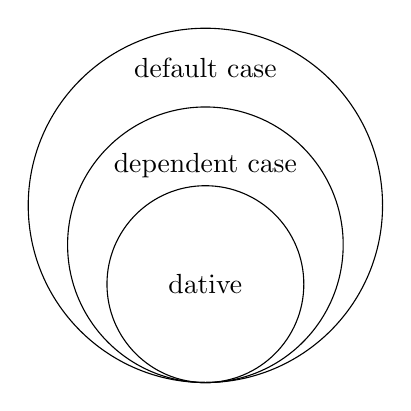
\begin{tikzpicture}
    \draw (0,1) circle (2.25);
    \draw (0,0.5) circle (1.75);
    \draw (0,0) circle (1.25);

    \node[] at (0,2.75) {default case};
    \node[] at (0,1.5) {dependent case};
    \node[] at (0,0) {dative};
  \end{tikzpicture}
  \caption{\posscitealt{bobaljik2006} schema}
  \label{fig:defdepdat}
\end{figure}

For this dissertation, this translates to this:

\begin{figure}[H]
  \centering
  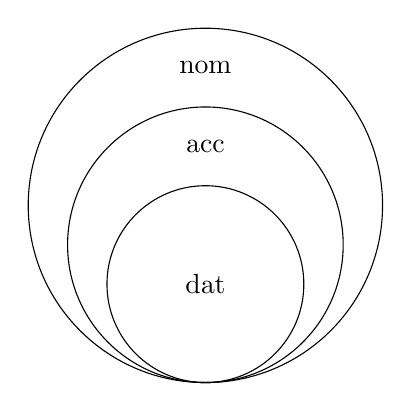
\begin{tikzpicture}
    \draw (0,1) circle (2.25);
    \draw (0,0.5) circle (1.75);
    \draw (0,0) circle (1.25);

    \node[] at (0,2.75) {\tsc{nom}};
    \node[] at (0,1.75) {\tsc{acc}};
    \node[] at (0,0) {\tsc{dat}};
  \end{tikzpicture}
  \label{fig:nomaccdat}
  \caption{Schema for this dissertation}
\end{figure}



\subsection{Relativization}

Keenan Comrie sub/obj/ind obj

Caha nom/acc/dat

In Malagasy, only subjects can be relativized. The basic word order of Malagasy is VOXS. a illustrates this point. a relative clause is formed by moving the head to the left, optionally adding the invariable relativizer \tit{izay}, and let the rest of the clause follow


RCs place
the head NP to the left, followed optionally by an invariable relativizer izay, followed
by the restricting clause with no pronoun in the NPrei position (Keenan (1972b))


\ex.
\ag. Nahita ny vehivavy ny mpianatra.\\
 saw the woman the student\\
 `The student saw the woman.'
\bg. ny mpianatra izay nahita ny vehivavy\\
 the student that saw the woman\\
 `the student that saw the woman'
\bg. *ny vehivavy izay nahita ny mpianatra\\
 the woman that saw the student\\
 `the woman that the student saw' \flushfill{Malagasy, \pgcitealt{keenan1977}{70}}

Objects can be passivized and then relativized (again relativization of a subject).

\ex.
\ag. Nohitan' ny mpianatra ny vehivavy.\\
 seen.\ac{pass} the student the woman\\
 `The woman was seen by the student.'
\bg. ny vehivavy izay nohitan' ny mpianatra\\
 the woman that seen.\ac{pass} the student\\
 `the woman that was seen by the student' \flushfill{Malagasy, \pgcitealt{keenan1977}{70}}

In Malay, subjects and objects can be relativized using \tit{yang}. Below I only give an example of a relativized object.

\exg. Ali bunoh ayam yang Aminah sedang memakan.\\
 Ali kill chicken that Aminah \ac{prog} eat\\
 `Ali killed the chicken that Aminah is eating.' \flushfill{Malay, \pgcitealt{keenan1977}{71}}

Indirect objects cannot be relativized in the same way.

\ex.
\ag. Ali beri {ubi kentang} itu kapada perempuan itu.\\
 Ali give potato the to woman the\\
 `Ali gave the potato to the woman.'
\bg. *perempuan yang Ali beri {ubi kentang} itu kapada\\
 woman that Ali give potato the to\\
\bg. *perempuan kapada yang Ali beri {ubi kentang} itu\\
 woman to who Ali give potato that\\ \flushfill{Malay, \pgcitealt{keenan1977}{71}}

A different construction is made.

\exg. perempuan yang menerima {ubi kentang} itu daripada Ali\\
 woman that received potato the from Ali\\
 `the woman that received the potato from Ali'\flushfill{Malay, \pgcitealt{keenan1977}{71}}

In Basque, subjects, objects and indirect objects can be relativized with the same strategy.

\ex.
\ag. Gizon-a-k emakume-a-ri liburu-a eman dio.\\
 man-\ac{def}-\ac{erg} woman-\ac{def}-\ac{dat} book-\ac{def}.\ac{acc} give has\\
 `The man has given the book to the woman.'
\bg. emakume-a-ri liburu-a eman dio-n gizon-a\\
 woman-\ac{def}-\ac{dat} book-\ac{def}.\ac{acc} give has-\ac{rel} man-\ac{def}\\
 `the man who has given the book to the woman'
\bg. gizon-a-k emakume-a-ri eman dio-n liburu-a\\
 man-\ac{def}-\ac{erg} woman-\ac{def}-\ac{dat} give has-\ac{rel} book-\ac{def}\\
 `the book that the man has given to the woman'
\bg. gizon-a-k liburu-a eman dio-n emakume-a\\
 man-\ac{def}-\ac{erg} book-\ac{def}.\ac{acc} give has-\ac{rel} woman-\ac{def}\\
 `the woman that the man has given the book to' \flushfill{Basque, \pgcitealt{keenan1977}{72}}




 \begin{table}[H]
   \center
   \caption {Relativization accessibility}
     \begin{tabular}{cccc}
       \toprule
             \multicolumn{3}{c}{relativization of}
           & \\
       \cmidrule{1-3}
             & direct
             & indirect
           & \\
             subject
             & object
             & object
           & example \\
       \cmidrule{1-3} \cmidrule{4-4}
             ✔
             & *
             & *
           & Malagasy \\
             ✔
             & ✔
             & *
           & Malay \\
             ✔
             & ✔
             & ✔
           & Basque \\
       \bottomrule
     \end{tabular}
 \end{table}






\section{Case in morphology}\label{sec:casemorphology}




\subsection{Syncretism patterns}

Icelandic: \pgcitealt{einarsson1949}{68}
Teribe: ?
Lavukaleve: Yvonne?
Khinalugh: Beata etc.


\begin{table}[H]
  \center
  \caption {Syncretism patterns}
    \begin{tabular}{cccccccc}
      \toprule
          \multicolumn{3}{c}{pattern}
            & \ac{nom}
            & \ac{acc}
            & \ac{dat}
            & translation
            & language \\
      \cmidrule(lr){1-3} \cmidrule(lr){4-6} \cmidrule(lr){7-7} \cmidrule(lr){8-8}
          A & A & A
            & \cellcolor{LG}\tbf{inu}
            & \cellcolor{LG}\tbf{inu}
            & \cellcolor{LG}\tbf{inu}
            & 2\ac{pl}
            & Lavukaleve \\
          A & B & B
            & ta
            & \cellcolor{LG}\tbf{bor}
            & \cellcolor{LG}\tbf{bor}
            & 1\ac{pl}
            & Teribe \\
          A & A & B
            & \cellcolor{LG}\tbf{það}
            & \cellcolor{LG}\tbf{það}
            & því
            & 3\ac{pl}.\ac{n}
            & Icelandic \\
          A & B & C
            & zɨ
            & jä
            & as(ɨr
            & 1\ac{sg}
            & Khinalugh \\
          A & B & A
            & \cellcolor{LG}
            &
            & \cellcolor{LG}
            &
            & not attested \\
      \bottomrule
    \end{tabular}
\end{table}







\ex. \ac{nom} < \ac{acc} < \ac{dat}


\subsection{Morphological containment}

\pgcitealt{nikolaeva1999}{16}

\begin{table}[H]
  \center
	\caption {Case containment in Khanty}
		\begin{tabular}{clll}
		\toprule
              & \ac{1}\ac{sg}
              & \ac{3}\ac{sg}
              & \ac{1}\ac{pl}                           \\
		          \cmidrule{2-4}
    \ac{nom}  & ma
              & luw
              & muŋ                                     \\
    \ac{acc}  & ma\tbf{:-ne:m}
              & luw\tbf{-e:l}
              & muŋ\tbf{-e:w}                           \\
    \ac{dat}  & ma\tbf{:-ne:m}-\tcol{DG}{\tbf{na}}
              & luw\tbf{-e:l}-\tcol{DG}{\tbf{na}}
              & muŋ\tbf{-e:w}-\tcol{DG}{\tbf{na}}  \\
		\bottomrule
		\end{tabular}
\end{table}


\pgcitealt{boretzky1994}{31-46}

\begin{table}[H]
  \center
	\caption {Case containment in Kalderaš Romani}
		\begin{tabular}{cllll}
		\toprule
              & `brother'
              & `brothers'
              & `girl'
              & `girls'                                   \\
		\cmidrule{2-5}
    \ac{nom}  & phral
              & phral-(á)
              & rakl-í
              & rakl-já                                   \\
    \ac{acc}  & phral-\tbf{és}
              & phral-\tbf{én}
              & rakl-\tbf{já}
              & rakl-já-\tbf{n}                           \\
    \ac{dat}  & phral-\tbf{és}-\tcol{DG}{\tbf{kə}}
              & phral-\tbf{én}-\tcol{DG}{\tbf{gə}}
              & rakl-\tbf{já}-\tcol{DG}{\tbf{kə}}
              & rakl-já-\tbf{n}-\tcol{DG}{\tbf{gə}}  \\
		\bottomrule
		\end{tabular}
\end{table}

\pgcitealt{gippert1987}{23-24}

\begin{table}[H]
  \center
	\caption {Case containment in West Tocharian}
		\begin{tabular}{cll}
		\toprule
              & `horses'
              & `men'                                  \\
		\cmidrule{2-3}
    \ac{nom}  & yakwi
              & eṅkwi                                  \\
    \ac{acc}  & yakwe-\tbf{ṃ}
              & eṅkwe-\tbf{ṃ}                          \\
    \ac{dat}  & yäkwe-\tbf{ṃ}-\tcol{DG}{\tbf{ts}}
              & eṅkwe-\tbf{ṃ}-\tcol{DG}{\tbf{ts}} \\
		\bottomrule
		\end{tabular}
\end{table}

\ex. \ac{nom} < \ac{acc} < \ac{dat}

\phantom{nom}




\section{A side note on the genitive}\label{sec:genitive}

\begin{itemize}
  \item possessive
  \item accessibility hierarchy
  \item not available
\end{itemize}
